\documentclass[11pt]{article}
\author{Hanxiao Du}
\title{Linear Regression}

\usepackage{geometry}
\geometry{margin=1in}
\usepackage{graphicx}
\graphicspath{ {./assets/} }


\begin{document}

\date{}
\maketitle
\noindent
\section{Introduction}
In statistics, linear regression is a linear approach to modeling the relationship between a scalar response (or dependent variable) and one or more explanatory variables (or independent variables). The case of one explanatory variable is called simple linear regression. For more than one explanatory variable, the process is called multiple linear regression.\\
\\
\section{Simple Linear Regression}
Given a data set $\{x_i,\ y_i\}_{i=1}^n$, where n is the amout of observations, $x_i$ is the i-th observation(with only one attribute) for $i=1,\ \cdots,\ n$ and $y_i$ is the corresponding label of the i-th observation for $i=1,\ \cdots,\ n$. Simple linear regression is of the from $y_i = w_0 + w_1 * x_i + \epsilon_i$, where $w_0$ is the intercept, $w_1$ is the slope and $\epsilon_i$ the noise of i-th observation. In this case, we would like to learn the parameters $w_0$ and $w_1$ from the observations.\\
\\
There are mainly two methods of estimating the parameters, one is called least-square estimation and the other one is Maximum-likelihood estimation. The former is a minimization problem and the latter is essentially the maximization dual of least-square estimation. Thus, the estimated values of parameters are the same no matter using either least-square estimation or MLE(Maximum likelihood estimation).\\
\\
For least-square estimation, the intention is to minimize the "loss"(or cost) of the model. The cost function we are using is the sum of squares of the distance between the data points and the regression line(see figure 1.1). The general idea of least-square estimation is that find such $w_0$ and $w_1$ so that the overall error is minimized(the sum of the length of red lines in figure 1.1).\\
\\
Notice that the loss function that we are using is the sum of squares of the lengths instead of just the sum of the lengths. This is mainly because the overall loss will usually be underestimated as a result of that some of the data points are above the regression line and some are below. The squareness makes the loss of each term positive and also it makes the derivative of the loss function much easier to be obtained as the purpose of finding minimum.\\
\begin{center}
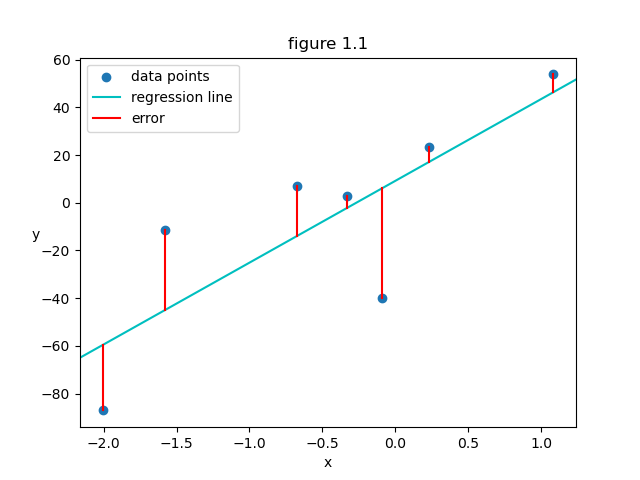
\includegraphics[scale=0.7]{figure_1.1}
\end{center}
In order to find the weights that minimize the loss function, firstly, we take the partial derivative of the loss function with respect of $w_0$. Let the loss function be denoted as $L(\{x_i,\ y_i\}_{i=1}^n) = \sum_{i=1}^n (y_i - (w_0+w_1*x_i))^2$.\\
$$\frac{\partial L}{\partial w_0} = -2\sum_{i=1}^n(y_i-(w_0+w_1*x_i))$$\\
Secondly, let $\frac{\partial L}{\partial w_0} = 0$, $$-2\sum_{i=1}^n (y_i - (w_0+w_1*x_i)) =0$$\\
$$w_0 = \bar{X} - w_1 * \bar{Y},$$ where $\bar{X}$ denotes the average of $\{x_i\}_{i=1}^n$ which is $\frac{1}{n}\sum_{i=1}^n x_i$ and $\bar{Y}$ denotes the average of $\{y_i\}_{i=1}^n$ which is $\frac{1}{n}\sum_{i=1}^n y_i$.\\
Now solving for $w_1$ with the same process shown above. We have $$\frac{\partial L}{\partial w_1} =  -2\sum_{i=1}^N(y_i-(w_0+w_1*x_i))*x_i$$\\
Let $\frac{\partial L}{\partial w_1} = 0$, $$-2\sum_{i=1}^N(y_i-(w_0+w_1*x_i))*x_i = 0$$
Plugging in $w_0 = \bar{Y} - w_1\bar{X}$, $$\sum_{i=1}^N x_i*y_i -\bar{Y}\sum_{i=1}^Nx_i+w_1\bar{X}\sum_{i=1}^N x_i - w_1\sum_{i=1}^N x_i^2 = 0$$\\
$$w_1 = \frac{\bar{Y}\sum_{i=1}^N x_i - \sum_{i=1}^N xi*yi}{\bar{X}\sum_{i=1}^N x_i-\sum_{i=1}^Nx_i^2}$$ and $w_0 = \bar{Y} - w_1\bar{X}$ are the solutions of $w_1$ and $w_0$ of least-square estimation.\\
\\
\\
Given a data set $\{x_i^1,\ x_i^2,\ \cdots,\ x_i^d,\ y_i\}_{i=1}^n$, where n is the amout of observations. Multiple linear regression is of the form $y_i = w_0 + w_1 * x_i^1 + w_2 * x_i^2 + \cdots + w_d * x_i^d + \epsilon_i$, where $x_i^j$ is the j-th attribute of the i-th observation, $y_i$ is the label of i-th observation, $w_0$ is the intercept ,$w_j$ is the weights of the j-th attribute for j=1, $\cdots$,d , d is the dimension(number of attributes) of the observations and $\epsilon_i$ the noise of i-th observation.\\
\\
In addition, for the sake of simplicity, we introduce the matrix form of linear regression. Let X denote the matrix of observations. X is of the form 
\end{document}